
\documentclass[a4paper]{scrreprt}
 
\usepackage[german]{babel}
\usepackage[utf8]{inputenc}
\usepackage[T1]{fontenc}
\usepackage{ae}

\usepackage[scaled]{helvet}
\renewcommand\familydefault{\sfdefault} 

\usepackage[onehalfspacing]{setspace}
\usepackage[scaled]{helvet}
\renewcommand*\familydefault{\sfdefault}

\usepackage[T1]{fontenc}
\usepackage{glossaries}
\usepackage{graphicx}
\usepackage[bookmarks,bookmarksnumbered]{hyperref}
\usepackage{float}
\usepackage[font={footnotesize}]{caption}
\usepackage{titlesec}

\setcounter{secnumdepth}{4}

\titleformat{\paragraph}
{\normalfont\normalsize\bfseries}{\theparagraph}{1em}{}
\titlespacing*{\paragraph}
{0pt}{3.25ex plus 1ex minus .2ex}{1.5ex plus .2ex}
\setlength{\parskip}{\baselineskip}%
\setlength{\parindent}{0pt}%

\setcounter{tocdepth}{1} 
\setcounter{secnumdepth}{2} 

\makenoidxglossaries

\newglossaryentry{Server}
{	name=Server,
	description={Ein Server (englisch server, wörtlich Diener oder Bediensteter, im weiteren Sinn auch Dienst) ist ein Computerprogramm oder ein Computer, der Computerfunktionalitäten wie Dienstprogramme, Daten oder andere Ressourcen bereitstellt, damit andere Computer oder Programme („Clients“) darauf zugreifen können}
}

\newglossaryentry{App}
{ 	name=App,
	plural=Apps,
	description={Als Mobile App (auf Deutsch meist in der Kurzform die App, eine Abkürzung für den Fachbegriff Applikation) wird eine Anwendungssoftware für Mobilgeräte beziehungsweise mobile Betriebssysteme bezeichnet}
}

\newglossaryentry{Nutzer}
{	name=Nutzer,
	description={Ein Benutzer (auch Endbenutzer, Bediener oder kurz Nutzer genannt sowie englisch User) ist eine Person, die ein Hilfs- oder Arbeitsmittel zur Erzielung eines Nutzens verwendet, beispielsweise für eine Zeitersparnis oder Kostensenkung}
}

\newglossaryentry{Desktop Anwendung}
{	name=Desktop Anwendung,
	plural=Desktop Anwendungen,
	description={Als Desktop Anwendungen (auch Anwendungsprogramm, kurz Anwendung oder Applikation; englisch application software, kurz App) werden Computerprogramme bezeichnet, die genutzt werden, um eine nützliche oder gewünschte nicht systemtechnische Funktionalität zu bearbeiten oder zu unterstützen. Sie dienen der „Lösung von Benutzerproblemen“}
}

\newglossaryentry{Drag and Drop}
{	name=Drag and Drop,
	description={Drag and Drop, oft auch Drag’n’Drop, deutsch „Ziehen und Ablegen“, ist eine Methode zur Bedienung grafischer Benutzeroberflächen von Rechnern durch das Bewegen grafischer Elemente mittels eines Zeigegerätes. Ein Element wie z. B. ein Piktogramm kann damit gezogen und über einem möglichen Ziel losgelassen werden. Dieses kann zum Beispiel markierter Text oder das Symbol einer Datei sein }
}

\newglossaryentry{Medikament}
{	name=Medikament,
	description={Arzneimittel oder gleichbedeutend Medikamente (lateinisch medicamentum „Heilmittel“) sind Stoffe oder Stoffzusammensetzungen, die „zur Heilung oder zur Verhütung menschlicher oder tierischer Krankheiten bestimmt sind“ oder sich dazu eignen, physiologische Funktionen zu beeinflussen oder eine medizinische Diagnose zu ermöglichen}
}

\newglossaryentry{NFC}
{ 	name=NFC,
	description={Die Nahfeldkommunikation (Near Field Communication, abgekürzt NFC) ist ein auf der RFID-Technik basierender internationaler Übertragungsstandard zum kontaktlosen Austausch von Daten per elektromagnetischer Induktion mittels loser gekoppelter Spulen über kurze Strecken von wenigen Zentimetern}
}

\newglossaryentry{Versichertennummer}
{ 	name=Versichertennummer,
	description={Die Krankenversichertennummer dient der Identifikation des Versicherten bei einer Krankenversicherung. Die Krankenversichertennummer wird benötigt, damit Leistungserbringer, z. B. Ärzte oder Zahnärzte ihre Leistungen mittels der Krankenversicherungskarte, über die Kassenärztlichen Vereinigungen, mit der zuständigen Krankenkasse abrechnen können}
}


\newglossaryentry{Bluetooth}
{	name=Bluetooth,
	description={Bluetooth ist ein in den 1990er Jahren durch die Bluetooth Special Interest Group (SIG) entwickelter Industriestandard gemäß IEEE 802.15.1 für die Datenübertragung zwischen Geräten über kurze Distanz per Funktechnik (WPAN). Dabei sind verbindungslose sowie verbindungsbehaftete Übertragungen von Punkt zu Punkt und Ad-hoc- oder Piconetze möglich}
}

\newglossaryentry{Pop-Up}
{	name=Pop-Up,
	description={Ein Pop-up (von englisch to pop up, „plötzlich auftauchen“) ist ein Element einer grafischen Benutzeroberfläche. In der Regel werden Pop-ups eingesetzt, um zusätzliche Inhalte anzuzeigen oder eine bestimmte Interaktion abzufragen. Typischerweise „springen“ Pop-ups auf und überdecken dabei andere Teile der Benutzeroberfläche}
}

\newglossaryentry{Cloud}
{	name=Cloud,
	description={Die Cloud ist keine physische Größe, sondern ein riesiges Netzwerk aus Remoteservern, die über die ganzen Welt verteilt aber miteinander verbunden sind, damit sie als ein einziges großes Ökosystem funktionieren können}
}

\newglossaryentry{Tab}
{	name=Tab,
	description={Eine Registerkarte, auch Reiter oder Tab genannt, ist ein Steuerelement einer grafischen Benutzeroberfläche, das einem Registerblatt aus Aktenschränken nachempfunden wurde }
}
 
\newglossaryentry{Arztbrief}
{	name=Arztbrief,
	plural=Arztbriefe,
	description={Der Arztbrief, oft synonym als Epikrise, Entlassungsbrief, Patientenbrief oder Befundbericht bezeichnet, ist ein Transferdokument für die Kommunikation zwischen Ärzten. Der Arztbrief gibt einen zusammenfassenden Überblick über den Status des Patienten bei der Entlassung, einen Rückblick über den Krankheitsverlauf, die veranlasste Therapie, eine Interpretation des Geschehens zum Krankheitsverlauf im speziellen Fall}
}

\newglossaryentry{Anamnese}
{	name=Anamnese,
	description={Die Anamnese (von altgriechisch anámnēsis, deutsch ‚Erinnerung‘) ist die professionelle Erfragung von potenziell medizinisch relevanten Informationen durch Fachpersonal (z. B. einen Arzt)}
}
 
\begin{document}
\begin{titlepage}
\begin{figure}[h]
	\vspace{-4cm}
	\hspace{-2cm}
	
\includegraphics[ width=0.3\textwidth]{Kit_Logo}
	\label{fig:Aufg03_1}
\end{figure}
	\vspace{1.5cm}
	\centering
	
\includegraphics[width=0.5\textwidth]{graphics/myMD_Logo}\par\vspace{0.5cm}
	{\Huge myMD \par}
	\vspace{2cm}
	{\scshape\Large Entwurf\par}
	\vspace{1cm}
	Praxis der Softwareentwicklung WS2017/2018 \par
	\vspace{2cm}
	{\Large\itshape Philipp Pelcz, Philipp Karcher, Jan-Luca Vettel\par}
	\vfill
	supervised by \par
	Marc Aurel Kiefer

	\vfill

% Bottom of the page
	{\large \today \par}
\end{titlepage}
 
% Platzierung des Inhaltsverzeichnisses
\tableofcontents
\addtocontents{toc}{\protect\enlargethispage{10cm}}

\chapter{Einleitung}
%TODO

 
\chapter{Systemaufbau}
\section{Systemarchitektur}
%TODO

\section{Subsysteme}
\subsection{View}
%TODO
\subsection{ViewModel}
%TODO
\subsection{Model}
%TODO Bild einfügen
Das Model enthält alle Klassen und Methoden zum Speichern, Laden, Ändern, Senden und Empfangen der medizinischen Daten des Benutzers. 

Das Paket \textbf{DataModel} enthält dabei die Objekte zur Modellierung der in der Applikation enthaltenen Daten. Um über Änderungen an diesen Daten informiert zu werden, kann sich eine Klasse durch Implementierung der \textbf{EntityObserver} Schnittstelle anmelden.

Die Speicherung dieser Daten geschieht über das Paket \textbf{DatabaseModel}. Außerdem 
können Daten über dieses Paket gesucht und abgefragt werden.

Für das Senden und Empfangen von Dateien ist das \textbf{TransmissionModel} Paket zuständig.

Da die Daten in einem anderen Format übertragen, als sie intern in der Applikation verwendet werden, muss das Paket \textbf{ParserModel} benutzt um zwischen den Formaten zu konvertieren.

Letztlich wird noch um plattformübergreifend auf das lokale Dateisystem zugreifen zu können das Paket \textbf{FileHelper} benötigt.

Um den Zugriff auf das Model zu vereinfachen wird das Fassaden Muster verwendet. Das Paket \textbf{ModelFacade} nimmt Anfragen an das Model entgegen und delegiert dann an die restlichen Pakete im Model.

\section{Subsystem-Schnittstellen}
\subsection{ModelInterface}
\subsubsection{TransmissionModelInterface}
%TODO
\subsubsection{DataModelInterface}
Hier sind die Schnittstellen der medizinischen Daten enthalten, die angezeigt werden sollen. Die hier aufgeführten Methoden umfassen daher das Abfragen von Informationen über die Daten aber auch einfache Operationen die auf diesen Daten ausgeführt werden, wie zum Beispiel das Ändern dieser Informationen.
\paragraph{IEntity}
%TODO Bild einfügen
\textbf{GetName() : string}\\
Gibt den Namen der Entität zurück.

\textbf{SetName(name : string) : void}\\
Setzt den Namen der Entität auf \textit{name}.

\paragraph{IData}
Die Schnittstelle \textbf{IData} erweitert \textbf{IEntity}.

%TODO Bild einfügen
\textbf{GetDate() : DateTime}\\
Gibt das Datum zurück, von dem die Daten stammen.

\textbf{GetSensitivity() : Sensitivity}\\
Gibt die Sensitivitätsstufe der Daten zurück.

\textbf{SetSensitivity(sensitivity : Sensitivity) : void}\\
Setzt die Sensitivitätsstufe der Daten auf \textit{sensitivity}.

\paragraph{IDoctorsLetter}
Die Schnittstelle \textbf{IDoctorsLetter} erweitert \textbf{IData}.

%TODO Bild einfügen
\textbf{GetDiagnosis() : string}\\
Gibt die Diagnose im Arztbrief zurück.

\textbf{GetDoctor() : IDoctor}\\
Gibt den Doktor zurück, von dem der Arztbrief stammt.

\textbf{GetMedication() : IList<IMedication>}\\
Gibt alle Medikationen zurück, die von diesem Arztbrief stammen.

\textbf{RemoveMedication(med : IMedication) : void}\\
Entfernt die Medikation \textit{med} aus der Liste der Medikationen die von diesem Arztbrief stammen.

\textbf{GetGroups() : IList<DoctorsLetterGroup>}\\
Gibt alle Gruppen von Arztbriefen zurück, in denen dieser Arztbrief enthalten ist.

\paragraph{IDoctorsLetterGroup}
Die Schnittstelle \textbf{IDoctorsLetter} erweitert \textbf{IData}.

%TODO Bild einfügen
\textbf{GetAll() : IList<IDoctorsLetter>}\\

\textbf{Add(letter : IDoctorsLetter) : void}\\

\textbf{Remove(letter : IDoctorsLetter) : void}\\

\textbf{GetLastDate() : DateTime}\\


\paragraph{IMedication}
Die Schnittstelle \textbf{IMedication} erweitert \textbf{IData}.

%TODO Bild einfügen
\textbf{SetDate(date : DateTime) : void}\\
Setzt das Datum an dem diese Medikation angefangen wurde auf das Datum \textit{date}.

\textbf{GetFrequency() : int}\\
Gibt zurück wie oft die Medikation in ihrem Intervall genommen werden soll.

\textbf{SetFrequency(freq : int) : void}\\
Setzt die Häufigkeit in der die Medikation in ihrem Intervall genommen werden soll auf \textit{freq}.

\textbf{GetInterval() : Interval}\\
Gibt zurück in welchem Zeitintervall die Medikation eingenommen werden soll. Das Intervall und die Häufigkeit zusammen ergeben dann eine tatsächliche Häufigkeit in der die Medikation eingenommen werden soll (z.B. 3 mal pro Tag).

\textbf{SetInterval(interval : Interval) : void}\\
Setzt das Zeitintervall in dem die Medikation eingenommen werden soll auf \textit{interval}.

\textbf{GetEndDate() : DateTime}\\
Gibt das Datum an dem die Medikation abgesetzt werden soll zurück.

\textbf{SetEndDate(date : DateTime) : void}\\
Setzt das Datum an dem die Medikation abgesetzt werden soll auf \textit{date}.

\textbf{DisattachFromLetter() : void}\\
Löst die Verbindung der Medikation zu ihrem Arztbrief auf.

\paragraph{IProfile}
Die Schnittstelle \textbf{IProfile} erweitert \textbf{IEntity}.

%TODO Bild einfügen
\textbf{GetInsuranceNumber() : string}\\
Gibt die Versicherungsnummer dieses Profils zurück.

\textbf{SetInsuranceNumber(number : string) : void}\\
Setzt die Versicherungsnummer dieses Profils auf \textit{number}.

\textbf{GetLastName() : string}\\
Gibt den Nachnamen dieses Profils zurück.

\textbf{SetLastName(name : string) : void}\\
Setzt den Nachnamen dieses Profils auf \textit{name}.

\textbf{GetBloodType() : BloodType}\\
Gibt die Blutgruppe dieses Profils zurück.

\textbf{SetBloodType(bloodType : BloodType) : void}\\
Setzt die Blutgruppe dieses Profils auf \textit{bloodType}.

\textbf{GetBirthDate() : DateTime}\\
Gibt das Geburtsdatum dieses Profils zurück.

\textbf{SetBirthDate(date : DateTime) : void}\\
Setzt das Geburtsdatum dieses Profils auf \textit{date}.

\paragraph{IDoctor}
Die Schnittstelle \textbf{IDoctor} erweitert \textbf{IEntity}.

%TODO Bild einfügen
\textbf{GetField() : string}\\
Gibt das Fachgebiet dieses Doktors zurück.

\textbf{SetField(field : string) : void}\\
Setzt das Fachgebiet dieses Doktors auf \textit{field}.


\paragraph{Enumerations}
Die Enumerationen \textit{Sensitivity}, \textit{Interval} und \textit{BloodType} müssen Subsystemen die auf die hier aufgeführten Daten zugreifen ebenfalls bekannt sein, um diese anzeigen zu können.

\subsubsection{ModelFacadeInterface}
%TODO Bild einfügen
Dies ist die Haupteinstiegsstelle für andere Subsysteme (hier nur das ViewModel) in das Model. Als Ein- und Ausgabeparameter werden die zuvor aufgeführten Schnittstellen verwendet. Alle komplexeren Operationen die nicht schon von diesen Schnittstellen übernommen werden, sind hier enthalten:

%TODO Datenübertragungsmethoden

\textbf{SetActiveProfile(profile : IProfile) : void}\\
Wechselt das aktive Profil zum Profil \textit{profile}.

\textbf{CreateEmptyProfile() : IProfile}\\
Legt ein neues Profil an, das noch keine Informationen und Daten enthält und gibt dieses zurück. Wechselt außerdem das aktive Profil zu diesem Profil.

\textbf{DeleteProfile(profile : IProfile) : void}\\
Löscht das Profil \textit{profile} und alle damit assoziierten Daten.

\textbf{GetAllDoctorsLetters() : IList<IDoctorsLetter>}\\
Fordert alle Arztbriefe des aktiven Profils an und gibt diese zurück.

\textbf{DeleteDoctorsLetter(letter : IDoctorsLetter) : void}\\
Löscht den Arztbrief \textit{letter} und alle Assoziationen zu ihm 

\textbf{GetAllMedications() : IList<IMedication>}\\
Fordert alle Medikationen des aktiven Profils an und gibt diese zurück.

\textbf{CreateEmptyMedication() : IMedication}\\
Legt eine neue Medikation an, die noch keine Informationen enthält und gibt diese zurück.

\textbf{DeleteMedication(medication : IMedication) : void}\\
Löscht die Medikation \textit{medication} und alle Assoziationen zu ihr.

\textbf{GetAllGroups() : IList<IDoctorsLetterGroup>}\\
Fordert alle Gruppen von Arztbriefen des aktiven Profils an und gibt diese zurück.

\textbf{CreateEmptyGroup() : IDoctorsLetterGroup}\\
Legt eine neue Gruppe von Arztbriefen an, die noch keine Arztbriefe enthält und gibt diese zurück.

\textbf{DeleteGroup(Group : DoctorsLetter) : void}\\
Löscht die Gruppe von Arztbiefen \textit{medication} und alle Assoziationen zu ihr. Die einzelnen Arztbriefe in der Gruppe selbst bleiben jedoch erhalten.

\chapter{Paketführer}

\section{Paketbeschreibung}
\subsection{View}
%TODO
\subsection{ViewModel}
%TODO
\subsection{Model}
%TODO

\section{Benutzt-Relation}
%TODO

\chapter{Klassenbeschreibung}
\section{View}
%TODO

\section{ViewModel}
%TODO

\section{Model}
\subsection{ModelFacade}
%TODO
\subsection{TransmissionModel}
%TODO
\subsection{DatabaseModel}
%TODO
\subsection{DataModel}
%TODO
\subsection{ParserModel}
%TODO
\subsection{FileHelper}
%TODO


\chapter{Daten}
%TODO

\chapter{Dynamik und Ablauf}
\section{Aktionen}
\newpage

%TODO

\begin{figure}
\section{UI-Navigation}
\centering
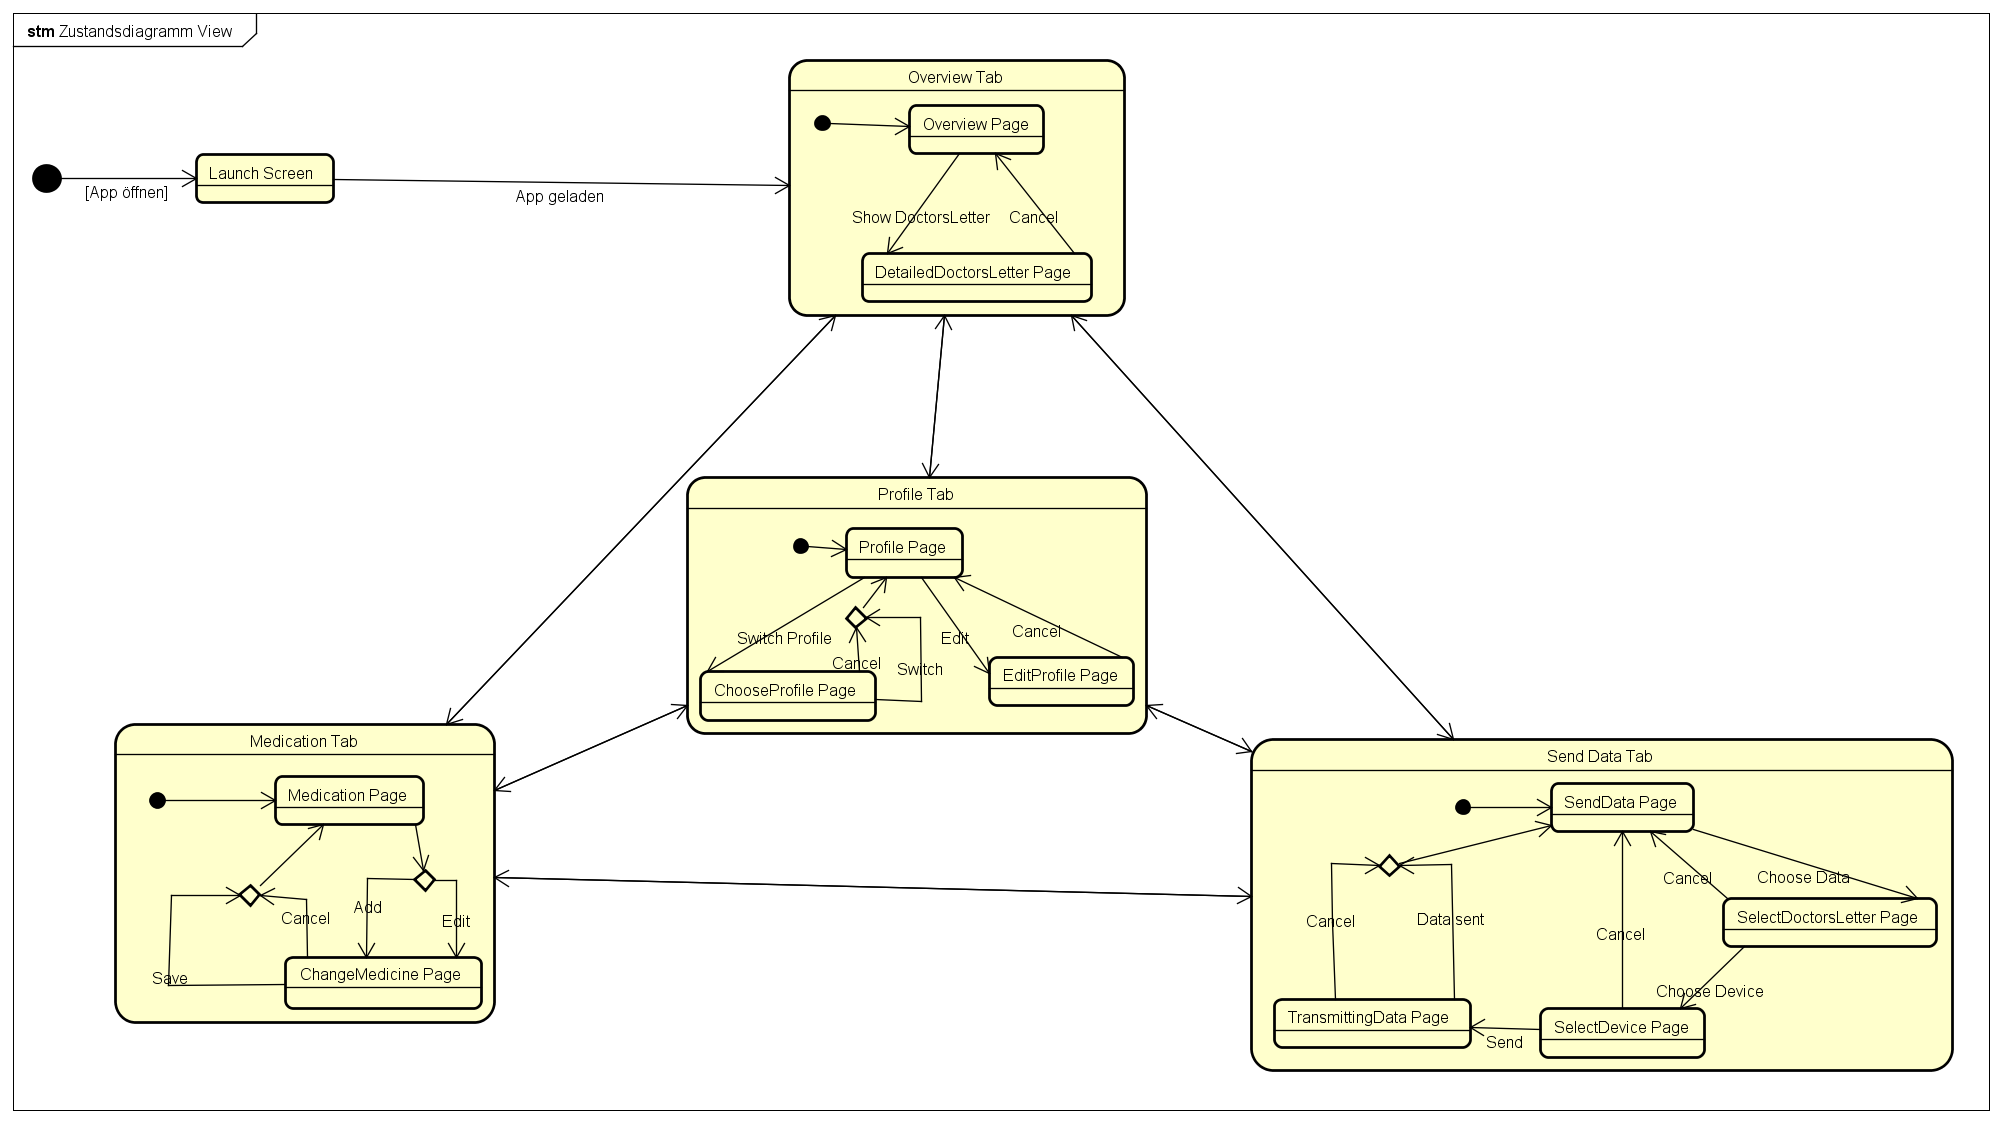
\includegraphics[width=0.9\textheight, angle=90]{graphics/Zustandsdiagramm_View}
\caption{Zustandsdiagramm der View}
\end{figure}
\begin{figure}
Die hauptsächliche Navigation in der Anwendung erfolgt über eine Tab Bar, die es dem Nutzer erlaubt, von jedem der vier Tabs in einen beliebigen anderen wechseln zu können. 
\\
\\
Startet der Nutzer die Anwendung zum ersten Mal, so gelangt er nach einer Begrüßung durch den Launch Screen zunächst in den Overview Tab.
Hier bietet sich ihm nun die Möglichkeit, durch das Auswählen eines beliebigen Arztbriefes in eine detaillierte Ansicht des Briefes zu gelangen.
Von hieraus gelangt der Nutzer nur durch einen Klick auf den Schließen Knopf zurück zur Overview Page.
\\
\\
Wechselt der Nutzer nun in den Medication Tab, gelangt er zunächst in die Medication Page. Diese stellt eine Übersicht über alle eingetragenen Medikationen dar. Über einen Hinzufügen Knopf gelangt man von dort aus in die ChangeMedicine Page, die das Anlegen einer neuen Medikation ermöglicht. Mit einem Klicken auf Speichern oder Abbrechen gelangt man wieder zurück zur Medication Page. Eine zweite Möglichkeit, die ChangeMedicine Page zu erreichen, stellt das Tippen auf einen beliebigen Eintrag der MedicationPage dar: Dadurch bietet sich die Möglichkeit, die vorhandenen Werte der Medikation anzupassen.
\\
\\
Der SendData Tab präsentiert dem Nutzer zunächst die SendData Page, von wo aus ein Tippen auf einen Knopf weiterleitet zur SelectDoctorsLetter Page, die es ermöglicht, die zu übertragenden Arztbriefe auszuwählen. Sind alle Dateien ausgewählt, gelangt der Nutzer über einen Knopf zur SelectDevice Page, wo er einen Empfänger auswählen kann. Hat er auch das erledigt, leitet ihn ein letzter Knopf zur TransmittingData Page weiter, die ihm einen Überblick über den Übertragungszustand bietet. Nach erfolgreicher Datenübertragung gelangt er über einen Knopf zurück zur SendData Page.
Alle der drei genannten Pages verfügung zudem über einen Cancel Button, der den Nutzer direkt zurück zur SendData Page leitet, und beispielsweise den Datenübertragungsvorgang abbricht.
\\
\\
Der letzte der vier Tabs, der Profile Tab, stellt dem Nutzer zunächst das aktuelle Profil in der Profil Page dar. Hier hat der Benutzer nun zwei Möglichkeiten: Entweder er entschließt sich zum Wechsel des aktiven Profils durch einen Knopfdruck Switch Profile, oder er möchte das aktuelle Profil editieren. 
Ersteres leitet ihn weiter zur ChooseProfile Page, wo er aus den gespeicherten Profilen zu einem beliebigen wechseln kann. Ein Speichern Knopf sichert die Änderung und leitet zurück zur Profile Page.
Möchte der Nutzer allerdings ein Profil editieren, erreicht er dies über einen Edit Knopf, der ihn zur EditProfile Page weiterleitet. Hier können entweder die eingetragenen Werte geändert und durch einen Speichern Knopf gesichert werden, oder durch man bricht den Vorgang durch einen Cancel Knopf ab. Beides leitet den Nutzer zurück zur ProfilePage.
\\
\\
Die Anwendung lässt sich zu jedem Zeitpunkt beenden. Aktive Datenübertragungsvorgänge werden dadurch jedoch beendet. Zudem gehen nichtgespeicherte Änderungen jeglicher Art verloren.
\end{figure}

\begin{figure}
\section{UI-Seiten}

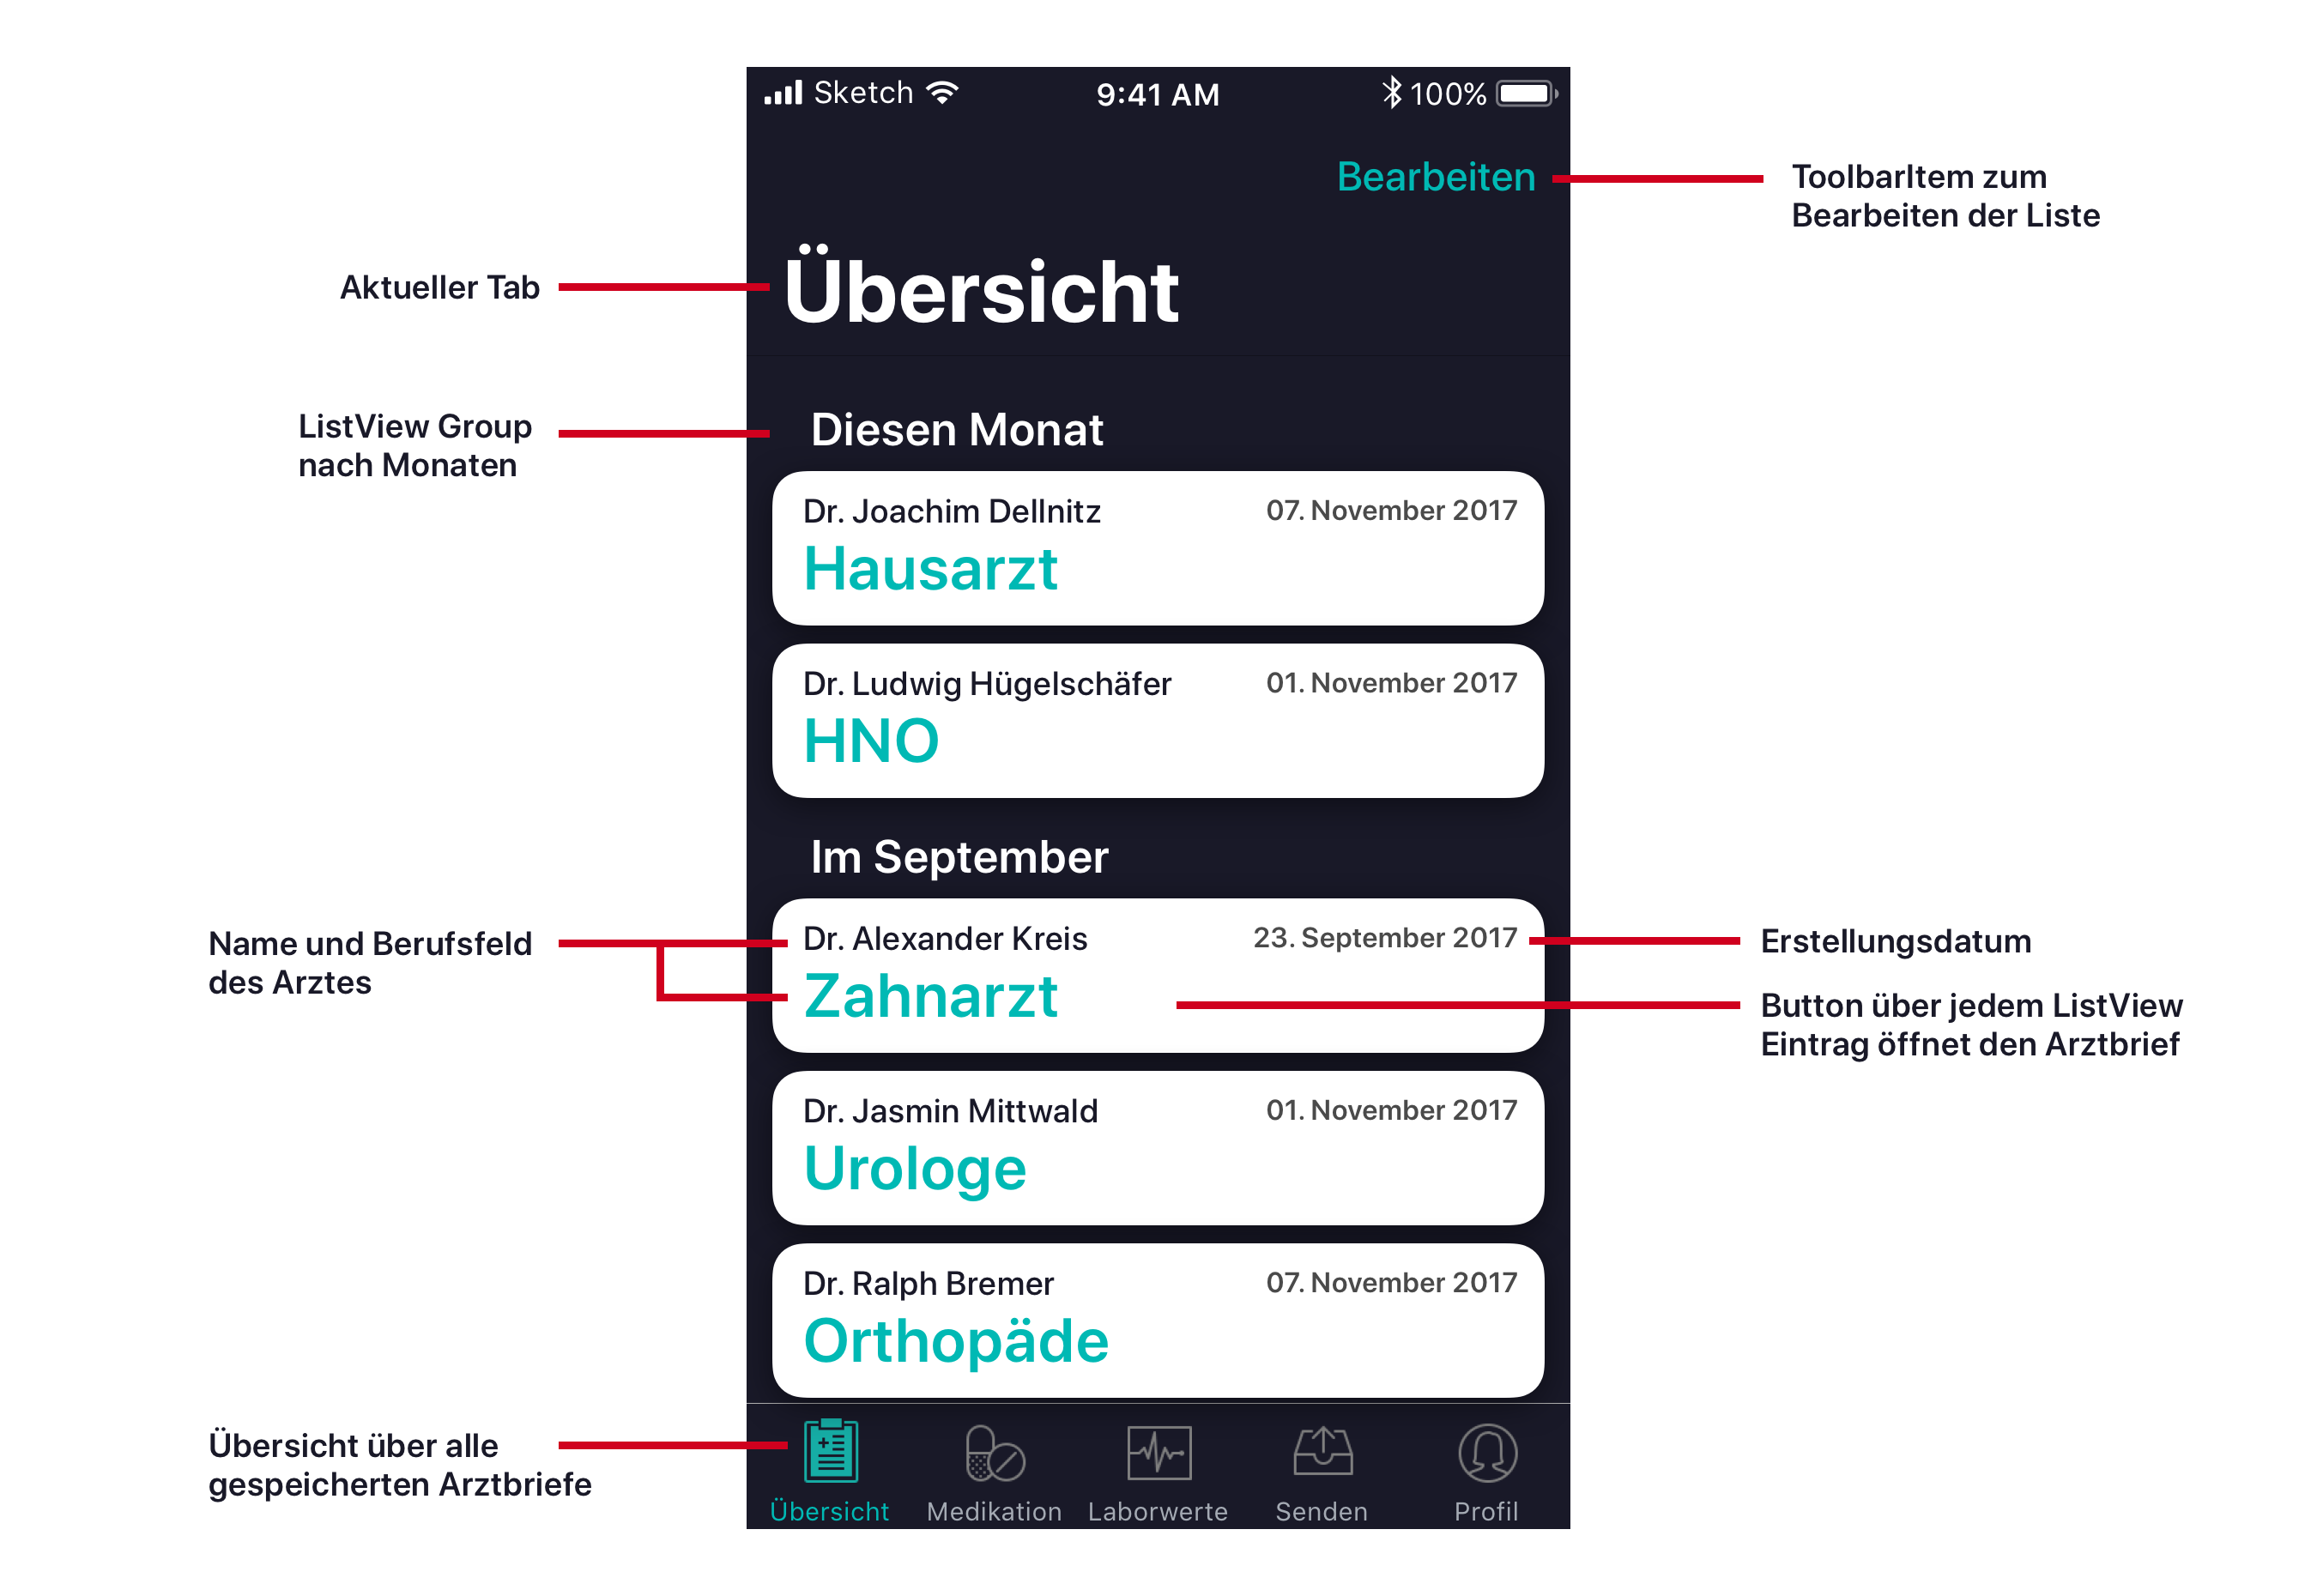
\includegraphics[width=1\textwidth]{graphics/UIDescriptions/OverviewDesc}
\caption{Beschreibung zum Tab "Übersicht"}
\vspace{0.5cm}
Wird die Anwendung geöffnet, wird dem Nutzer zunächst eine Übersicht all seiner gespeicherten Arztbriefe angezeigt (Overview Page). Die Arztbriefe sind hierbei chronologisch absteigend in einer ListView angeordnet. Tippt der Nutzer einen Listeneintrag an, öffnet sich eine ausführliche Ansicht des Arztbriefes.
\end{figure}

\begin{figure}
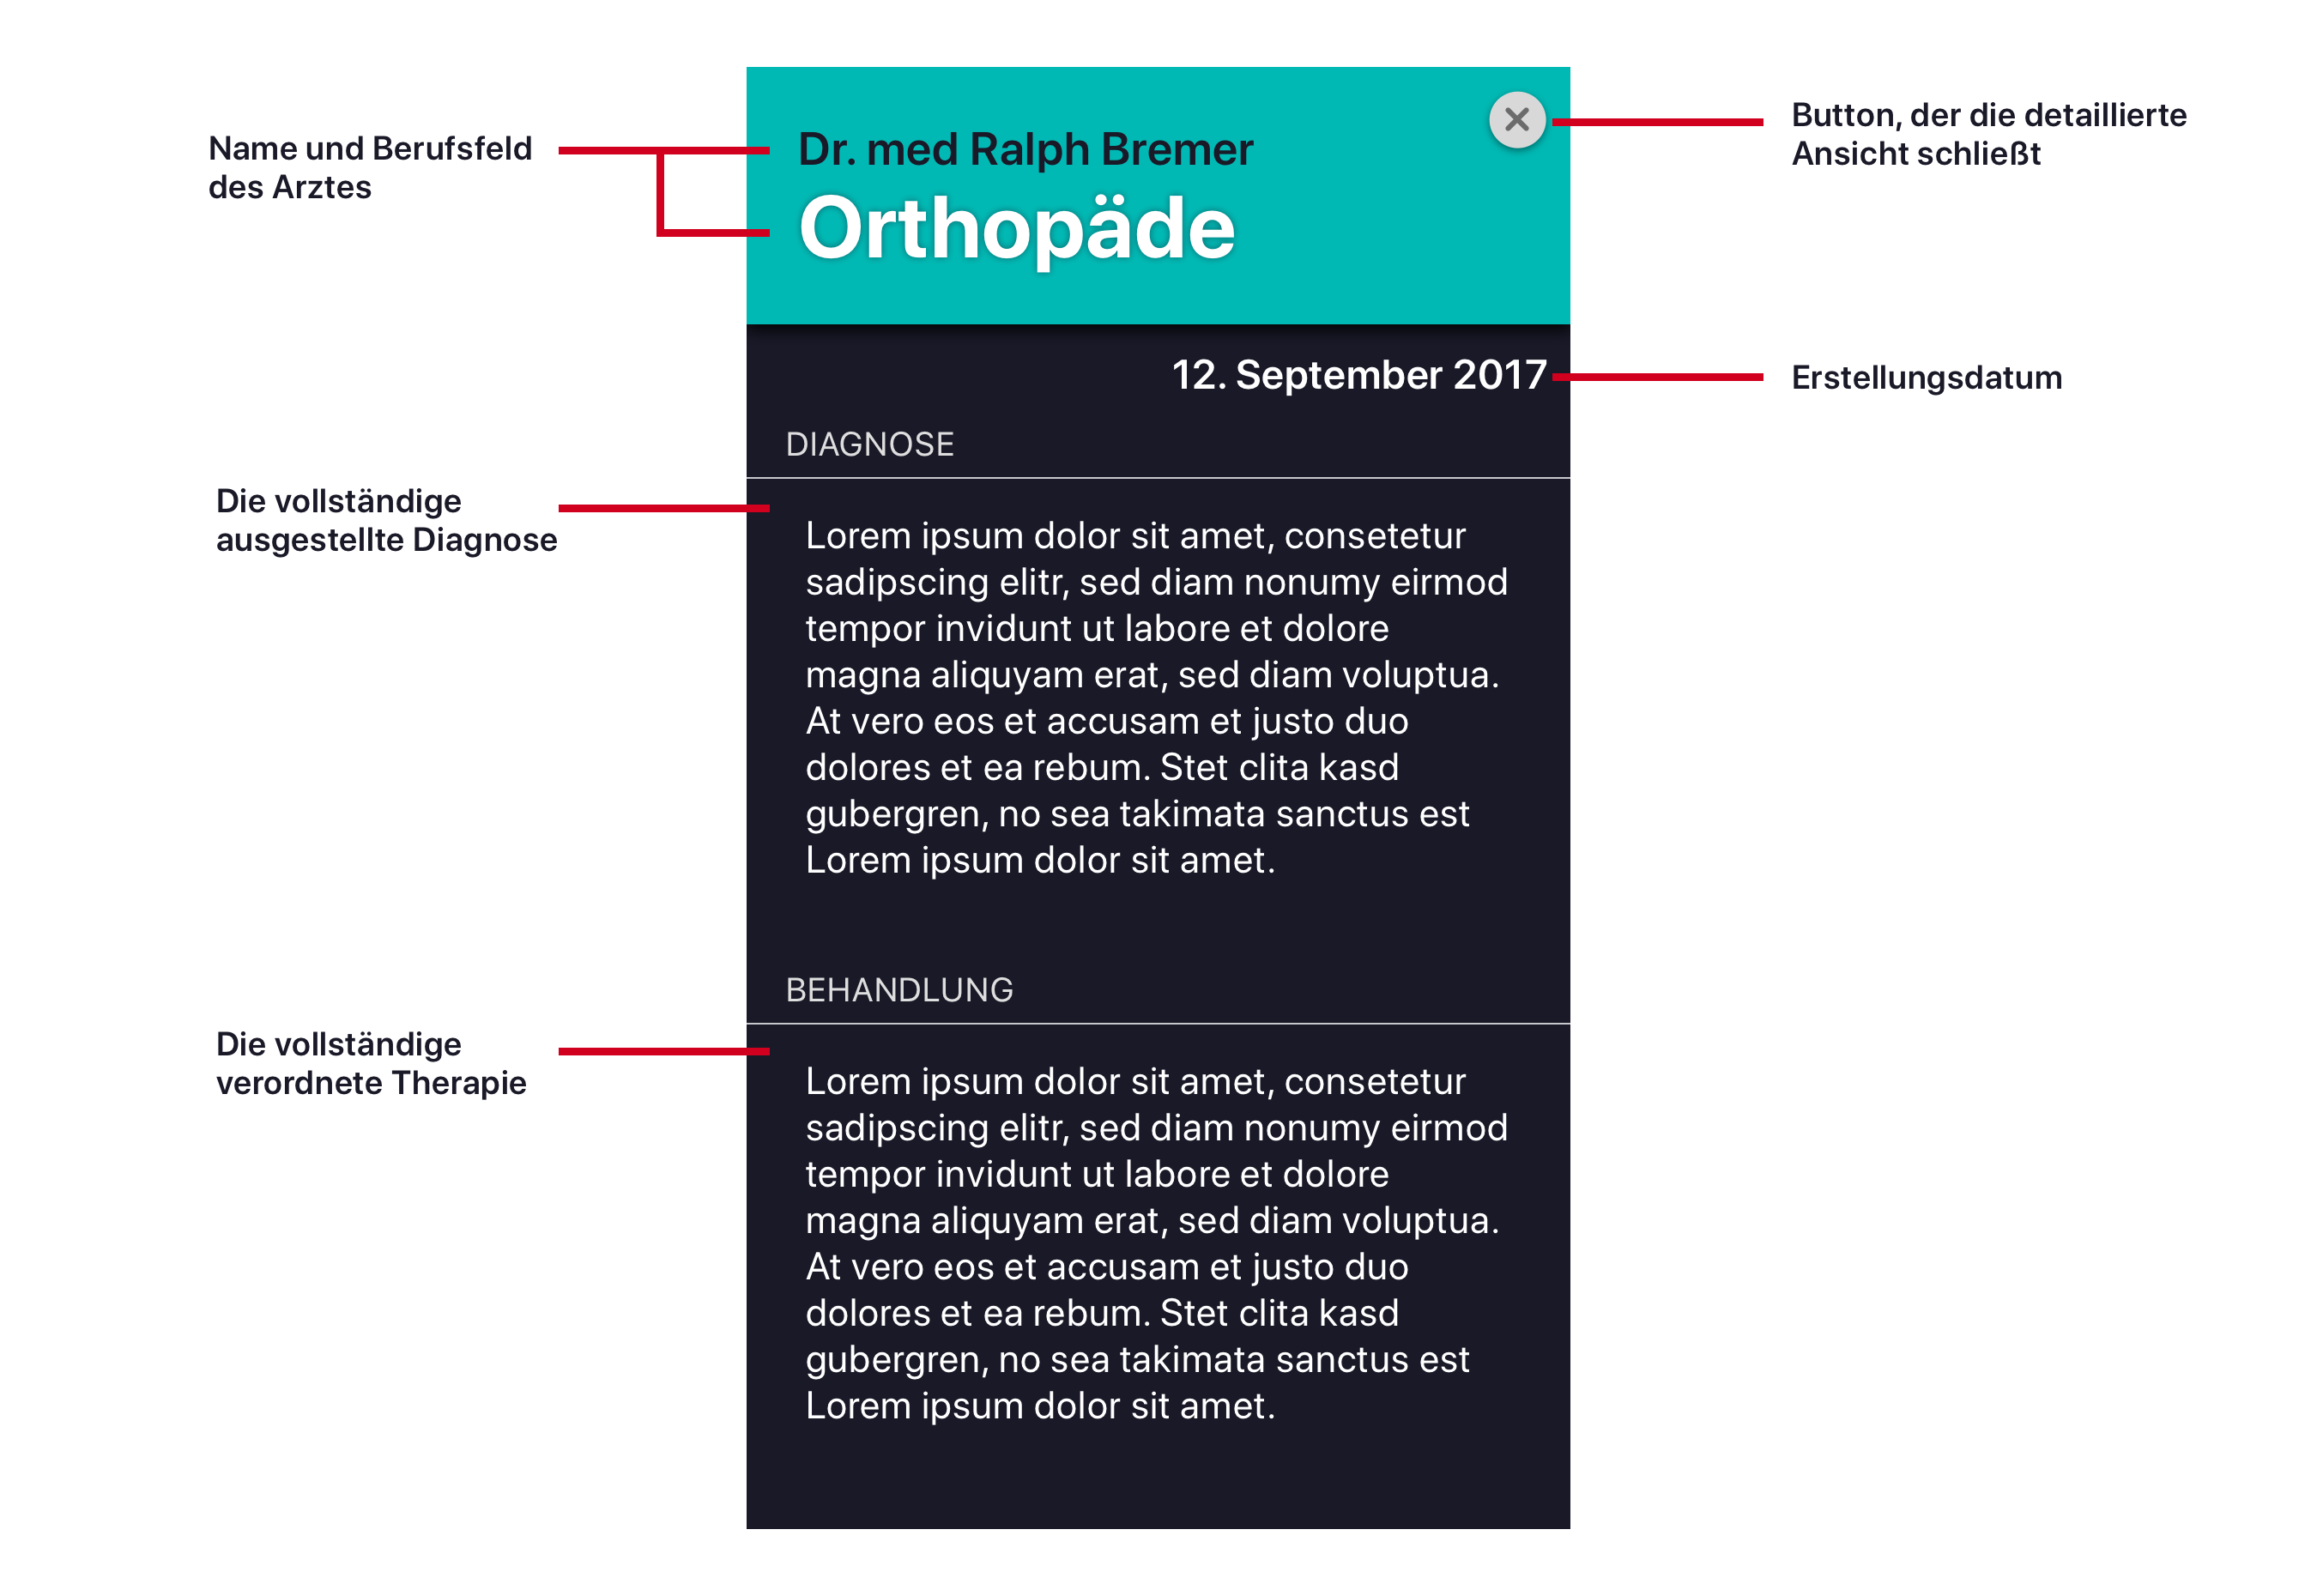
\includegraphics[width=1\textwidth]{graphics/UIDescriptions/DetailedDLDesc}
\end{figure}

\chapter{Klassendiagramm}
%TODO


\printnoidxglossaries

% Abbildungsverzeichnis
\listoffigures
 
\end{document}
